\chapter{РАЗРАБОТКА ПРОГРАММНОЙ ПЛАТФОРМЫ}

В данной главе описываются нюансы проектирования и разработки программного робототехнического фреймворка. В дальнейшем фреймворк будет именоваться RRC (Register, Run, Communicate). В первой части главы описываются подходы для достижения поставленных требований к производительности и масштабируемости системы, применяемые в данной работе. Вторая часть содержит описание архитектуры синхронной версии фреймворка. В последней части говорится об особенностях реализации асинхронного робототехнического фреймворка. Библиотека реализованна на языке программирования C++ стандарта ISO/IEC 14882:2014 с использованием системы кроссплатформенной сборки CMake 3.7 \cite{martin2015mastering}. Исходный код распространяется под лицензией Apache 2.0 \cite{rosen2005open}.

\section{Исследование способов проектирования модульных систем}

При разработке высокопроизводительного фреймворка был использован язык программирования C++ стандарта 2014 года по ряду причин. Популярные интерпретируемые языки при разработке ядра системы не рассматривались из-за дополнительных затрат вычислительных ресурсов на интерпретацию кода. При разработке робототехнических систем активно используется низкоуровневое взаимодействие с аппаратной частью или с операционной системой поэтому для разработки программного обеспечания для РТК желательно использовать язык пригодный для системного программирования. Для решения подобных задач на данный момент конкурентом C-подобным языкам является язык rust \cite{matsakis2014rust}, но на данный момент язык не имеет достаточного количество инструментов для разработки из-за чего от него пришлось отказаться. Язык С++ стандарта 2014 года имеет множество встроенных средств, позволяющих отказаться от использования библиотеки Boost. Boost – наиболее распространенная библиотека для расширения возможностей языка C++, включающая в себя огромное количество реализаций различных программных инструментов: от алгоритмов до метапрограммирования. Отказ от использования данной библиотеки позволит избавиться от большой зависимости и значительно облегчит платформу и ее развертывание. В языке C++ имеется встроенная поддержка многопоточности, что позволяет реализовать необходимые алгоритмы, такие как потокобезопасные контейнеры, управление многопоточным исполнением, синхронизация передаваемых данных и другие. Также с введением 11-го стандарта в языке C++ появилась поддержка ссылок на неименованные значения (rvalues), что позволяет использовать конструкторы перемещения вместо конструкторов копирования, значительно оптимизируя работу с памятью, что активно используется в работе.

Далее под модулем будет подразумеваться группа методов, которая принимает определенный набор данных и решает заданный набор задач независимо от конфигурации системы. Ядром системы является компонет, отвечающий за порядок исполнение модулей и задает фиксированный набор механизмов для коммуникации между ними. Каждый модуль может получать информацию о конфигурации системы и взаимодействовать с другими компонентами системы только через унифицированный интерфейс ядра.

\subsection{Модели исполнения}

В данном разделе рассмотренны синхронные и асинхронные модели исполнения и будут проанализированны их слабые и сильные стороны при разработке модульных многопоточных приложений.

Современные стандарты языка C++ после введения шаблонов с переменным количеством типов (variadic templates) и лямбда-функций активно используют функциональные объекты и различные приемы, взятые из функциональных языков, которые позволяют существенно уменьшить количество классов при использовании стандартных шаблонов проектирования. Нововведения позволяют существенно упростить разработку асинхронных приложений за счет использования высокоуровневых оберток вокруг функций и функциональных объектов (std::function). В основе реализации данного класса лежит паттерн type erasure. Его предназначение заключается в том, что различные сущности (объекты, указатели и пр.) скрываются за одним интерфейсом, которые предоставляют сходные возможности. Функциональный объект отвечает за хранение данных, поэтому имплементация интерфейса объекта создается и хранится в куче (heap). Узким местом такой реализации являются затраты на дополнительное аллоцирование памяти.

% Более подробное описание 

% Синхронная модель
В синхронном подходе требуется задать определенный интерфейс модуля, который будет последовательно выполнять определенную группу задач. Каждый модуль имеет входные точки: методы, в которых заключена вся логика обработки событий, полученных из ядра системы.

\begin{figure}[h]
    \centering{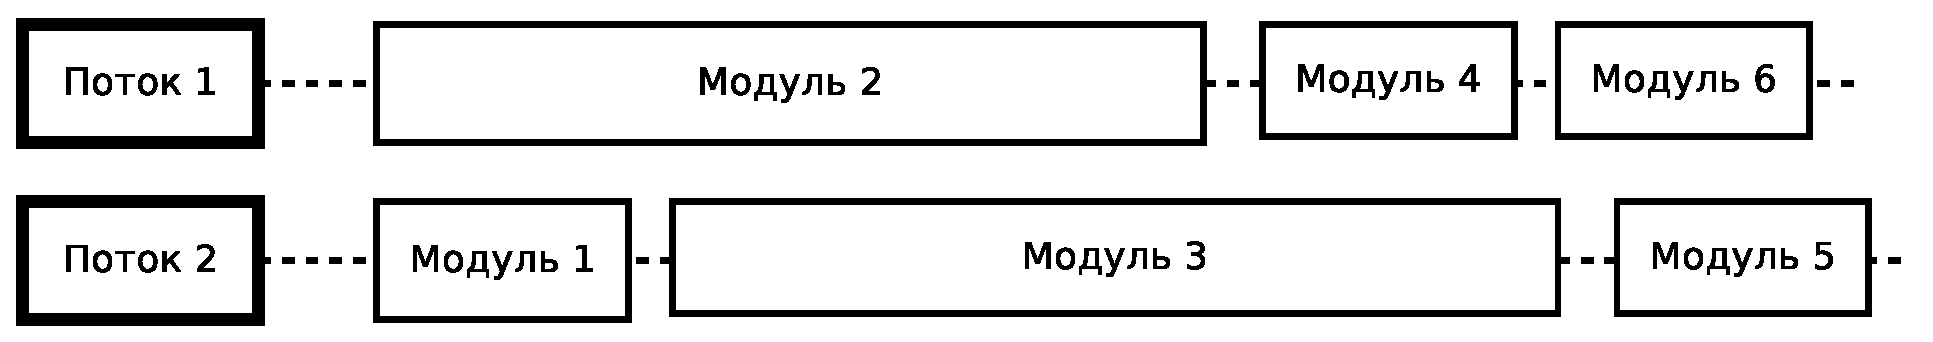
\includegraphics[width=1\linewidth]{2_1_1_sync}}
    \caption{Синхронное исполнение модулей в двух потоках}
    \label{im:2_1_1_sync}
\end{figure}

На рис. \ref{im:2_1_1_sync} изображена временная диаграмма обработки событий в двух потоках для синхронной системы. Этот график иллюстрирует типичную проблему данного подхода, когда несколько модулей имеют большое количество обработчиков входных данных (модули 2 и 3), из-за чего другие модули не имеют возможности продолжать обработку. Данная проблема может быть решена несколькими путями. В ROS данная проблема не возникает из-за того, что для каждого модуля создается отдельный процесс и используется системный планировщик задач для распределения нагрузки. Данный подход прямо зависит от реализации планировщика операционной системы, для которой разрабатывается фреймворк, а следовательно снижается переносимость кода. Другой вариант решения проблемы подразумевает разработчику модуля самостоятельно контролировать процессорное время, которое использует отдельный модуль, что существенно усложняет процесс разработки.

Так же синхронная модель исполнения подразумевает последовательную проверку входящих событий, что может привести к дополнительным вычислительным затратам при отсутствии входящих данных при большом количестве обработчиков событий.

При этом у синхронный подход позволяет исключить гонку за данные при обновлении модулей в многопоточных системах, из-за чего можно не беспокоиться об обеспечении потокобезопасности при проектировании модуля, если ядро системы предоставляет такую модель исполнения.

% Асинхронная модель
Асинхронная модель исполнения предоставляет более гибкий способ разработки модулей. В основе данного подхода лежит отложенное исполнение кода и получение уведомлений о событиях в системе за счет функций обратного вызова. Каждый модуль можно разбить на цепочки небольших задач, которые добавляются в глобальную очередь и выполняются по мере выполнения других задач, что позволяет равномерно распределить процессорные ресурсы между потоками.

В данной работе ядро системы было реализованно с использованием как синхронного, так и асинхронного подхода для сравнения производительности и способов дальнейшего расширения функциональности системы.

\subsection{Примитивы межпоточной синхронизации}

Многопроцессное и многопоточное программирование является очень мощным инструментом для организации модульных приложений. Помимо хорошей масштабируемости такой подход позволяет эффективнее использовать возможности современных многоядерных аппаратных вычислительных устройств за счет одновременного исполнения различных частей кода.

В данной работе исследование сконцентрированно на разработки модульной системы и коммуникации между модулями с искользованием lock-free алгоритмов. Как следует из названия, данные потокобезопасные контейнеры реализованы без использования мьютексов – взаимных исключений для обеспечения синхронизации при работе с несколькими потоками. Использование такого подхода позволяет значительно повысить скорость выполнения программы. Такие контейнеры соответствуют предполагаемой архитектуре программной платформы, поскольку в разрабатываемой платформе возможна ситуация MPMC (Multiple Producer Multiple Consumer) – данные в контейнер могут записываться из нескольких мест и считываться из нескольких мест. Использование контейнеров с блокирующей синхронизацией в таких случаях отрицательно сказывается на скорости работы программы при одновременном доступе к одной критической секции из разных потоков. Возможность применения таких контейнеров без использования сторонних библиотек обусловлена наличием необходимых для их реализации механизмов в 11-м стандарте языка С++.

В работе \cite{syzovalgorithm} рассматривается алгоритм для передачи большого количества данных через UDP протокол в высоконагруженной многопоточной системе. В данной работе используется высокопроизводиетльная реализация очереди без блокировок с открытым исходным кодом <<moodycamel ConcurrentQueue>>. В данной работе предлагается использовать данную реализацию очереди для повышения быстройдействия в многопоточной среде. Ниже представленны графики тестирование производительности добавления элементов в очередь (рис. \ref{im:2_1_2_dequeue}) и получения элементов из очереди (рис. \ref{im:2_1_3_enqueue}), взятые с сайта разработчика. Тестирование производительности на процессоре Intel Atom z530 выдавало схожие соотношения результатов.

\begin{figure}[h]
    \centering{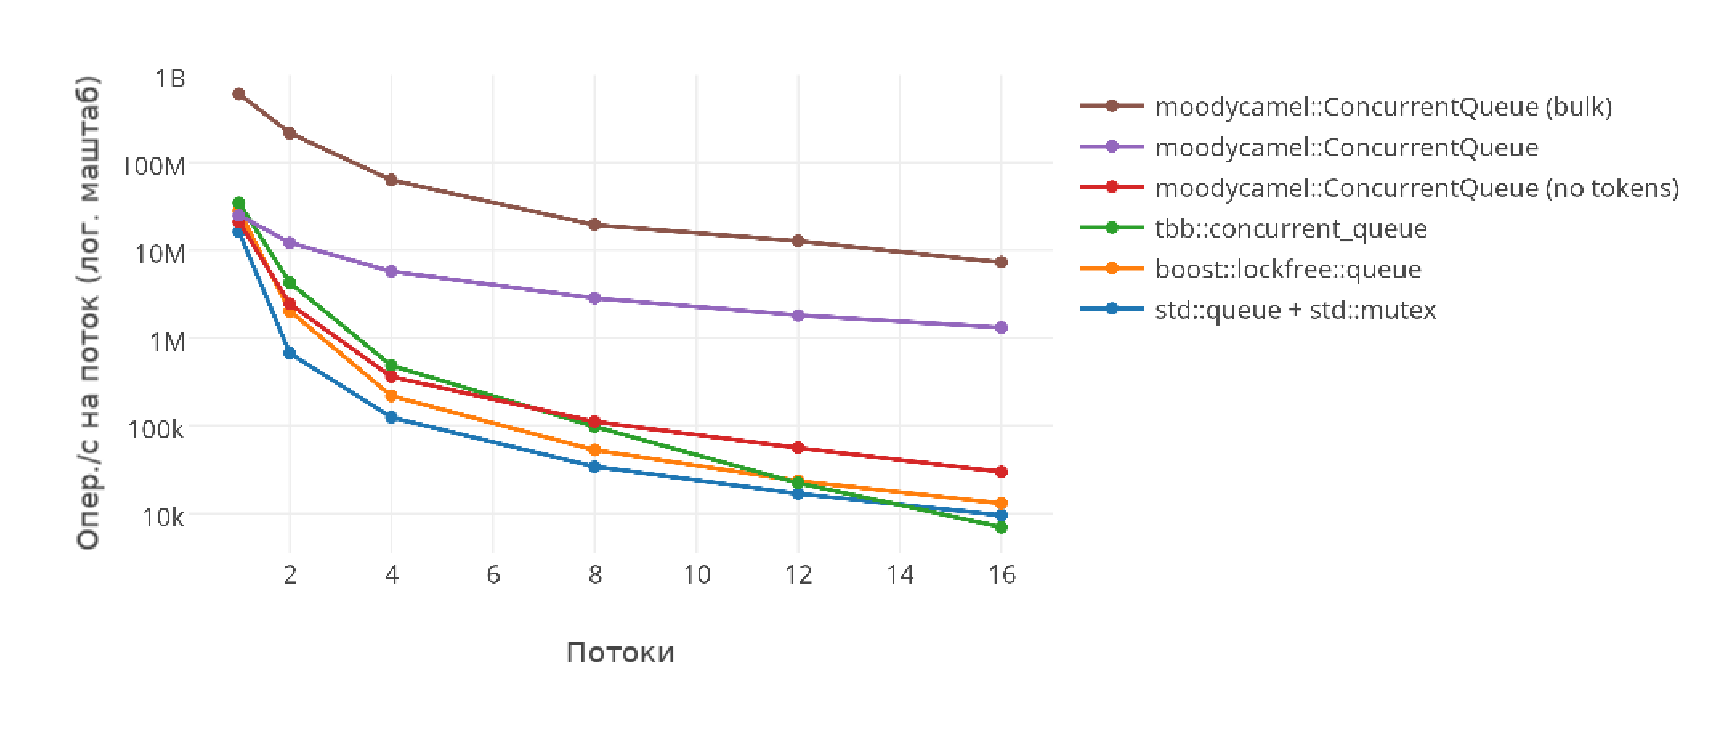
\includegraphics[width=1\linewidth]{2_1_2_dequeue}}
    \caption{Производительность получения элементов из очереди}
    \label{im:2_1_2_dequeue}
\end{figure}

\begin{figure}[h]
    \centering{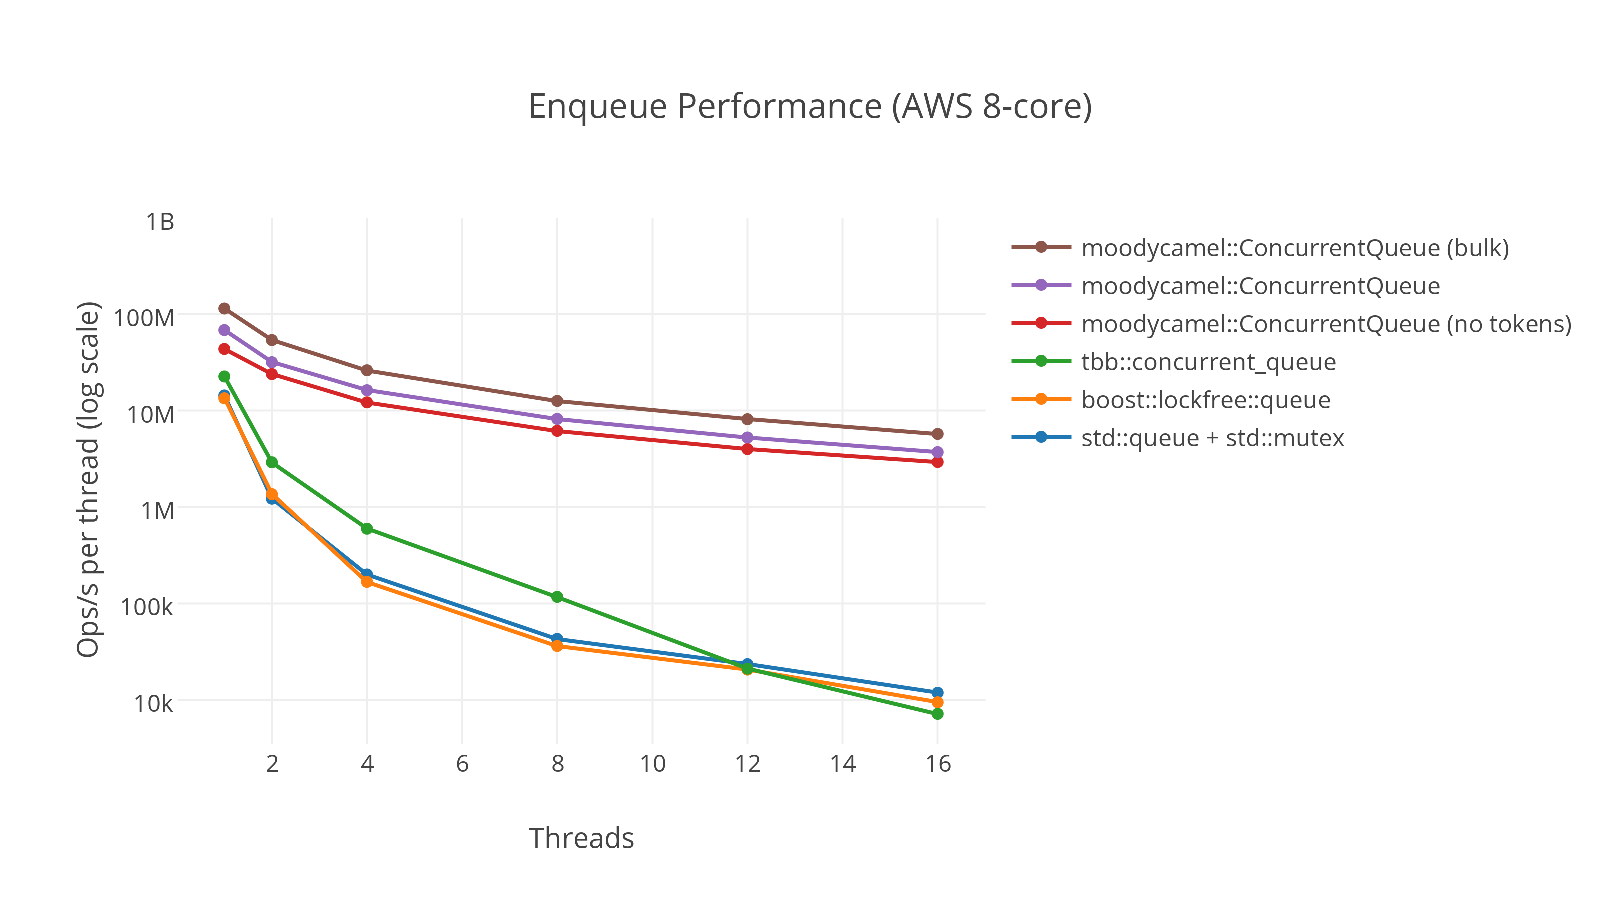
\includegraphics[width=1\linewidth]{2_1_3_enqueue}}
    \caption{Производительность добавления элементов в очередь}
    \label{im:2_1_3_enqueue}
\end{figure}

\subsection{Алгоритмы сериализации}

При проектировании механизмов межмодульной коммуникации предполагается возможность использования системного ввода/вывода для взаимодействия с системой через сетевые протоколы или для записи сообщений на диск и повторного воспроизведения передаваемых данных в соответствующем порядке для отладки системы или иного сценария, подразумевающего подобное взаимодействие с операционной системой.

Сериализация - это процесс перевода какой-либо структуры данных в последовательность битов. Восстановление начальной структуры данных из сериализованной последовательности битов называется десериализацией.

В работе \cite{sumaray2012comparison} производится сравнение популярных форматов сериализации (XML, JSON, Protobuf, Thrift) при использовании на мобильных платформах. Из данной работы интерес представляют замеры производительности и объем потребляемой памяти для хранения структур данных. Результаты исследования показывают явное преимущество в этих двух аспектах у бинарных форматов сериализации Protobuf и Thrift. Человекочитаемые форматы XML и JSON позволяют упростить отладку системы, но из-за их избыточности в данной работе дальше рассматриваться не будут и дальнейшее исследование будет направленно в сторону бинарных форматов представления данных.

В работе \cite{zaluzhnyi2016serialization} исследуются алгоритмы сериализации и десериализации для высокопроизводительных вычислительных систем. Самые лучше результаты показывают алгоритмы Cap'n Proto и Google Flat Buffers, которые используют алгоритмы десериализации без копирования (zero-copy deserialization). Поскольку десериализация занимает пренебрежимо малое процессорное время, данные в таком формате можно передавать внутри системы сразу в сериализованном виде.

В связи с отсутствием зависимостей и поддержки большого количества языков (C, С++, Java Python, Go, JavaScript) и платформ  в данной работе при проектировании систем обмена сообщениями будет использованны реализации Protocol Buffers и Flat Buffers. В данных решениях каждая структура данных описывается в отдельном файле (schema) на специальном языке разметки. Для генерации програмнного кода для описанных структур используется сторонняя утилита соответствующая для каждой из библиотек. Google Protocol Buffers позиционируется как компактный (memory efficient) инструмент для сериализации и десерелиализации данных. Компактность достигается за счет использования varint-подобных алгоритмов сжатия для целых чисел. Google Flat Buffers проектировался как аналог Protocol Buffers с уклоном в эффективное использование памяти для повышения быстродействия в играх реального времени. 

% Наработки по сериализатору

\section{Проектирование синхронного фреймворка}

Один из основных подходов, используемых при разработке платформы – это максимальная гибкость и расширяемость. В платформе используется абстракция – механизм, представляющая собой и на деле некий механизм, ответственный за определенную задачу синхронизации внутри платформы. При желании, разработчик, использующий платформу может для разных задач использовать готовые механизмы, но если считает, что они ему не подходят, то может добавлять свои механизмы, расширяя функционал платформы. В дальнейшем все вызовы будут обработаны в одном потоке, что исключает гонку за данные.

Продемонстрировать гибкость платформы можно наглядно на следующем примере: в платформе есть механизм, ответственный за запуск и исполнение всех модулей в системе; есть несколько вариантов этого механизма – обычный линейный, многопоточный, многопоточный с использованием пула потоков. При использовании системы на различных процессорах – одноядерных или многоядерных имеет смысл использовать различные режимы исполнения соответственно, чтобы исключить затраты на лишнюю синхронизацию и обеспечить максимальную производительность. Так, например, нет смысла запускать многопоточный режим на старом одноядерном процессоре, и в ту же очередь нет смысла не использовать возможность распараллеливания на многоядерных процессорах. Гибкость и расширяемость описываемой платформы позволяет подстроить ее под необходимую среду, в которой ей придется работать.

В данной реализации под механизмами будет подразумеваться класс-обертка вокруг потоконебезопасного класса, которая инкапсулирует все вызовы к данному классу в функциональный объект и помещает его в потокобезопасную очередь. Использование механизма отложенных синхронизаций позволяет избавиться от проблем зацикливания при ситуации, например, когда какой-нибудь модуль отправляет сообщения сам себе. Также, позволяет с легкостью подобрать нужную реализацию очереди под конкретную ситуацию. В асинхронной версии библиотеки структура механизма отличается от описанной в данном разделе.

Ниже, на рис. \ref{im:2_2_1_sync}, представлена схема синхронного прототипа ядра системы. Данная диаграмма классов включает только основной набор классов, которые демонстрируют механику взаимодействия между отдельными компонентами системы:

\begin{figure}[h]
    \centering{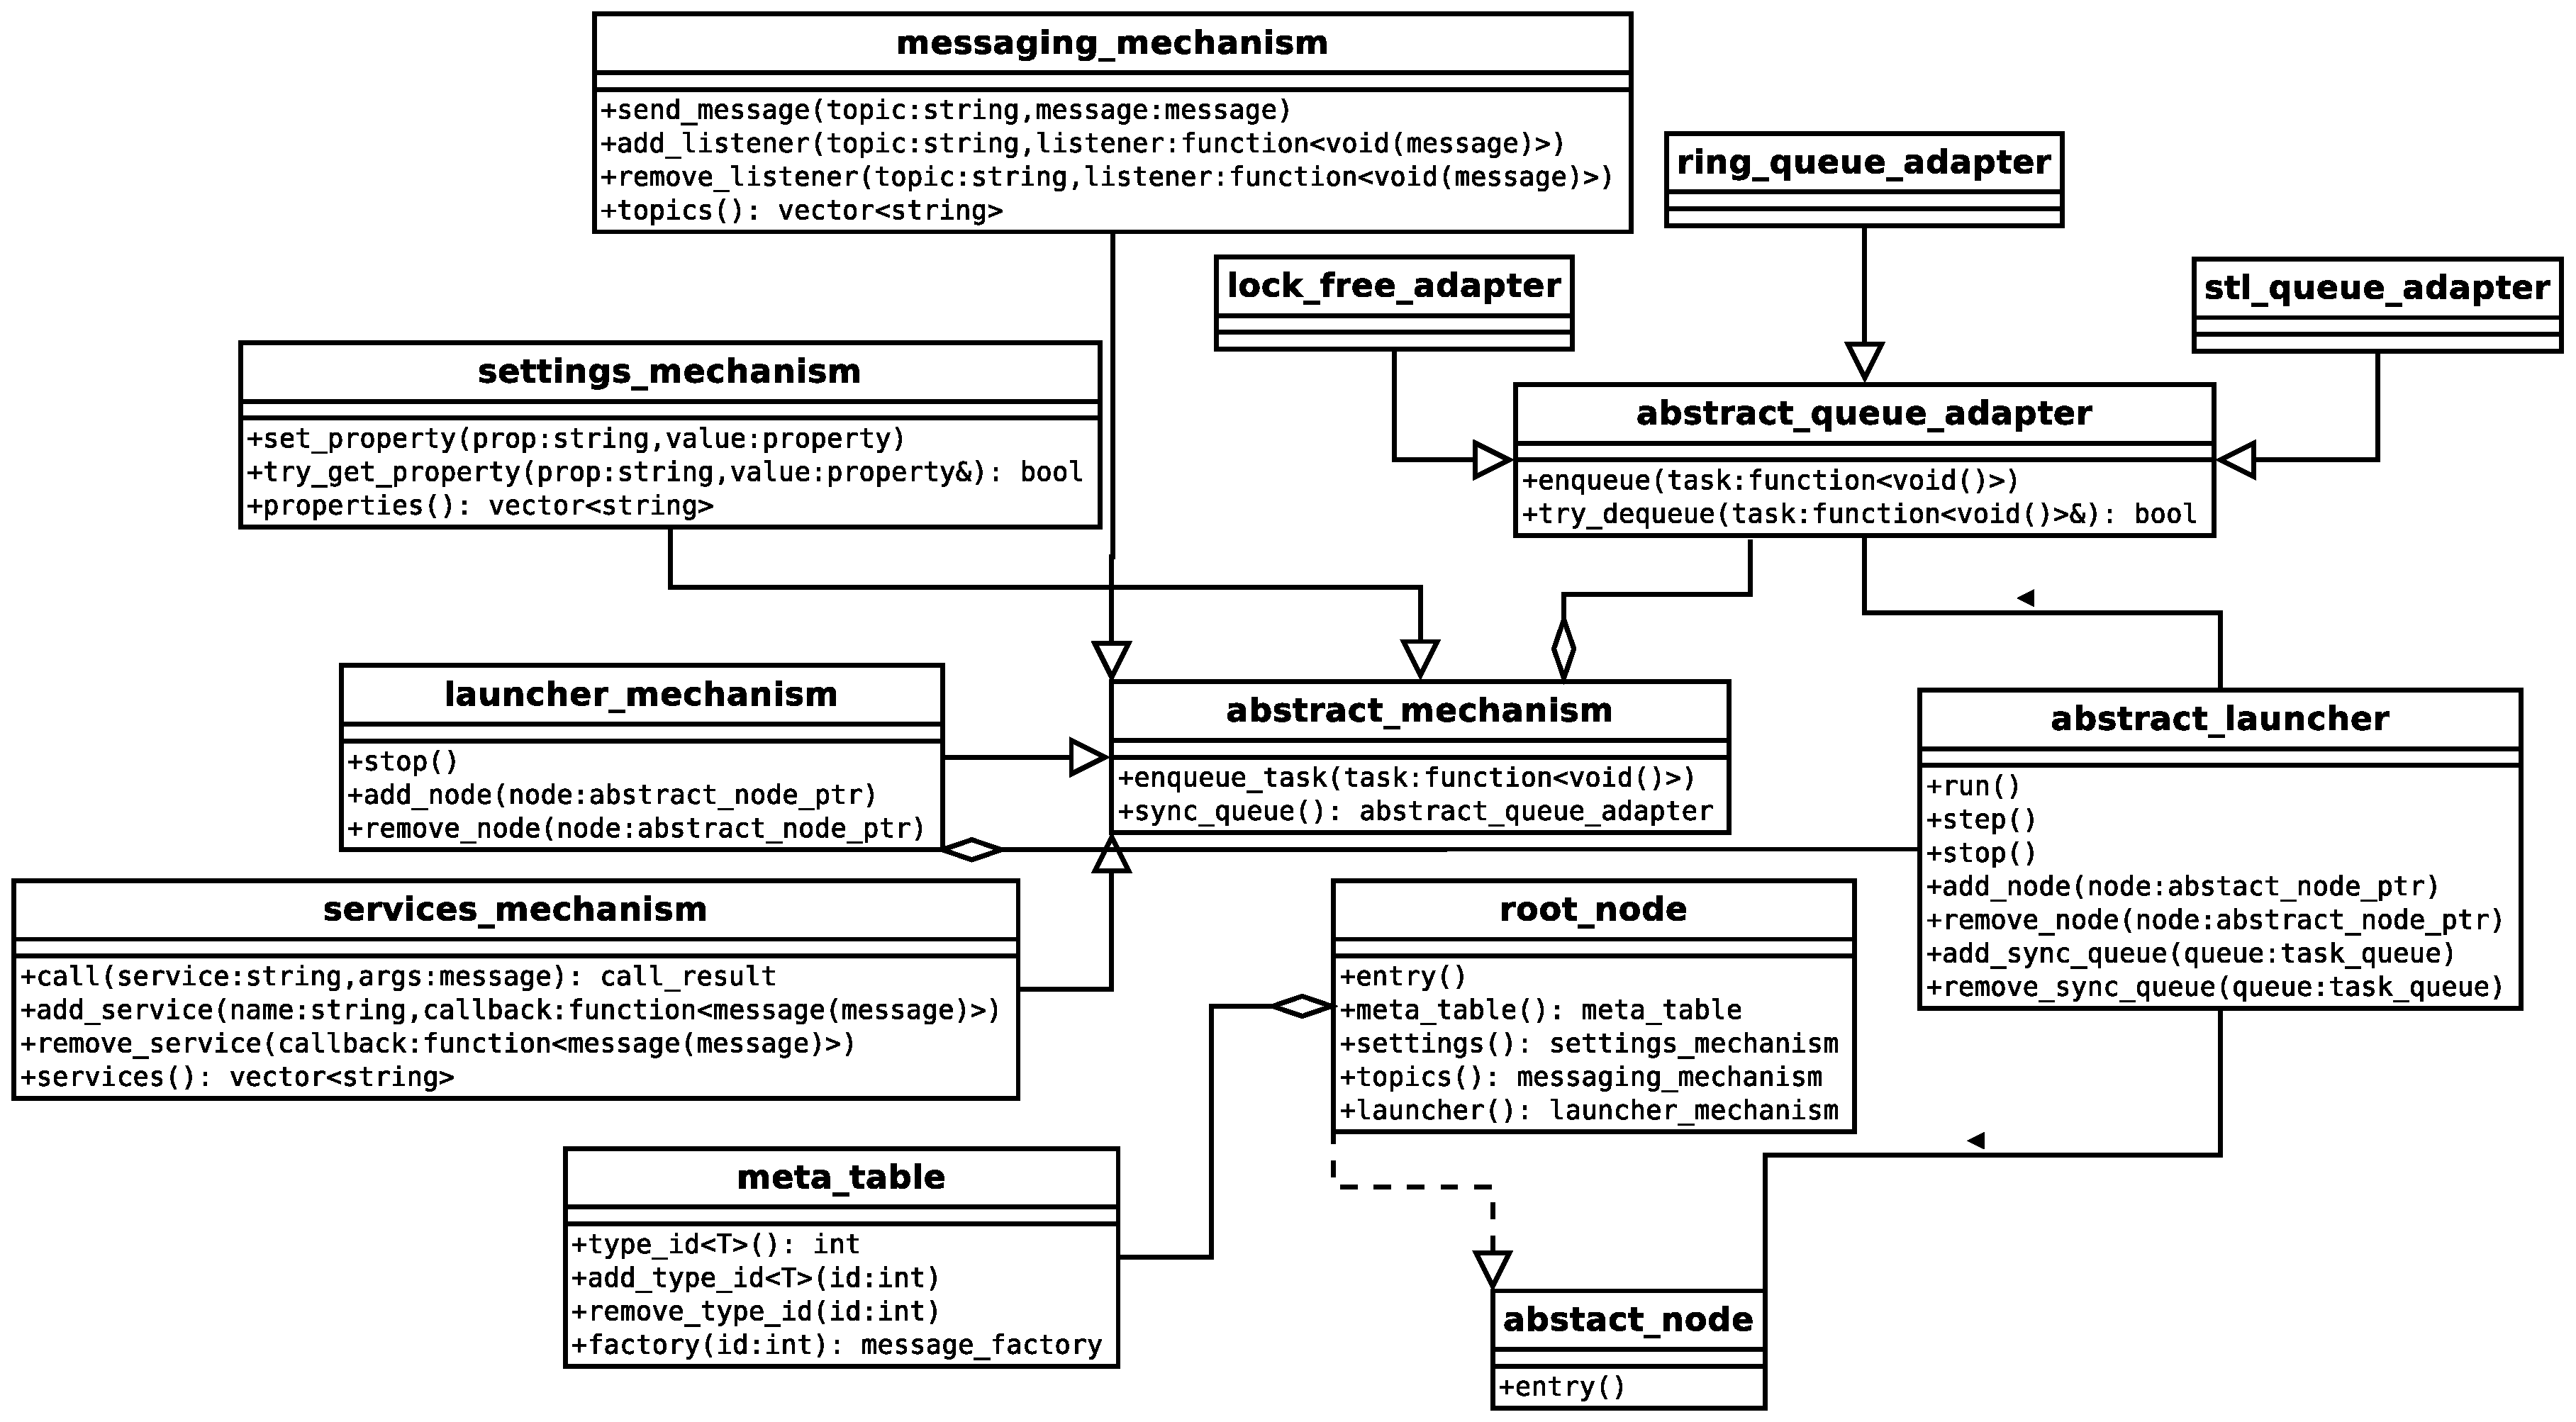
\includegraphics[width=1\linewidth]{2_2_1_sync}}
    \caption{Диаграмма классов синхронной версии фреймворка}
    \label{im:2_2_1_sync}
\end{figure}

\textit{abstract\_launcher} --- интерфейс исполняющего класса. Реализация данного класса должна хранить указатели на модули и очереди синхронизаций и обеспечивать требуемый порядок исполнения, например, последовательно в одном потоке или с использованием пула потоков.

\textit{abstract\_queue\_adapter} --- интерфейс компонента, необходимого для обеспечения отложенной синхронизации. Он передает все задачи по синхронизации на определенные очереди. Адаптер предоставляет единый интерфейс для добавления и получения элементов из очереди. Его возможные реализации:

\textit{stl\_queue\_adapter} --- компонент, необходимый для работы с очередью из стандартной библиотеки c++ STL. В данном классе не используются блокировки для повышения производительности на одноядерных системах

\textit{lock\_free\_adapter} --- компонент, необходимый для работы с lock-free(без использования мъютексов) очередью. В проекте используется реализация очереди Камерона Десрочерза (Cameron Desrochers).

\textit{ring\_queue\_adapter} --- компонент, необходимый для работы с  циклической очередью фиксированного размера.

\textit{abstract\_node} --- интерфейс, позволяющий создавать независимые компоненты системы --- модули, каждый из которых может быть ответственнен за свой конкретный функционал. Модули не знают о существовании других модулей, то есть, они на самом деле, полностью независимы друг от друга. Из взаимодействие и исполнение обеспечено ядром системы. Такой подход к созданию этой абстракции также позволяет переиспользовать разработанные на ее основе модули при различных конфигурациях описываемой робототехнической платформы, а так же позволяет исполнять каждый модуль в отдельном потоке без дополнительных затрат процессорного времени на синхронизацию. 

\textit{abstract\_mechanism} --- абстрактный класс для компонентов системы, обеспечивающих какой-либо потокобезопасный вид взаимодействия между модулями и с ядром системы. Класс содержит потокобезопасную очередь функциональных объектов, куда помещаются все вызовы к базовому классу. Для функционирования механизма Указатель на очередь должен быть зарегистрирован в экземпляре класса abstract\_launcher.

\textit{launcher\_mechanism} --- компонет, реализующий интерфейс abstract\_mechanism, обеспечивающий взаимодействий с конкретной реализацией abstarct\_launcher, позволяет добавлять и удалять модули, запускать и останавливать систему.

\textit{messaging\_mechanism} --- компонет, реализующий интерфейс abstract\_mechanism, обеспечивающий возможность коммуникации и обмена данными между модулями путем отправки сообщений. Данный механизм реализован с использованием паттерна <<издатель-подписчик>>. Экземпляр <<слушателя>> добавляется в список к именованному <<топику>>, куда в дальнейшем любой модуль может отправлять отправлять сообщения. Данный механизм реализован по аналогии с системой рассылки сообщений в ROS.

\textit{services\_mechanism} --- компонет, реализующий интерфейс abstract\_mechanism, обеспечивающий возможность запуска требуемых методов по их имени. Вызовы происходят в неблокирующем режиме, поэтому система позволяет отправить несколько запросов до получения ответа. Аргументы метода передаются в структуре сообщения. Результат выполнения будет записан в объект результата после выполнения функции. 

\textit{meta\_table} --- класс, который содержит информацию для идентификации сообщений. В данной реализации использовалась библиотека google protocol buffers. Поскольку в данной библиотеке используется не тривиальный алгоритм сериализации и десериализации, сообщения внутри системы передаются в <<сыром>> виде для уменьшения дополнительных нагрузок на систему. При регистрации нового типа сообщений так же создается экземпляр фабрики для сообщений, который позволяет при получении сериализированных данных верифицировать их и создать экземпляр сообщения.

Следует так же уделить внимание классу сообщений \textit{message}. В данной реализации, как было сказанно ранее, используется библиотке google protocol buffers для генерации сериализируемых сообщений. Сериализация необходима, например, для передачи сообщения через сетевой протокол. Сообщения хранятся и передаются внутри системы через умные указатели (\textit{std::shared\_pointer}) на экземпляр структуры, которая хранит данные. Данный прием позволяет передавать сообщения внутри системы без дополнительных затрат на копирование данных, а так же автоматически освобождать занятые ресурсы памяти, что дает существенный прирост в производительности всей системы при рассылке сообщений нескольким <<слушателям>>.

По умолчанию в системе реализован класс \textit{abstract\_launcher}, который поочередно запускает обработку модулей и стадию синхронизации. Такой порядок исполенения позволяет исключить гонку за данные при многопоточном исполнении, а следовательно упростить структуру модулей в случае, если модуль не создает собственного потока исполнения. На рис. \ref{im:2_2_2_sequence_diag} представленна диаграмма последовательностей, в которой изображен сценарий коммуникации модулей с ядром системы (механизмами синхронизации).

\begin{figure}[h]
    \centering{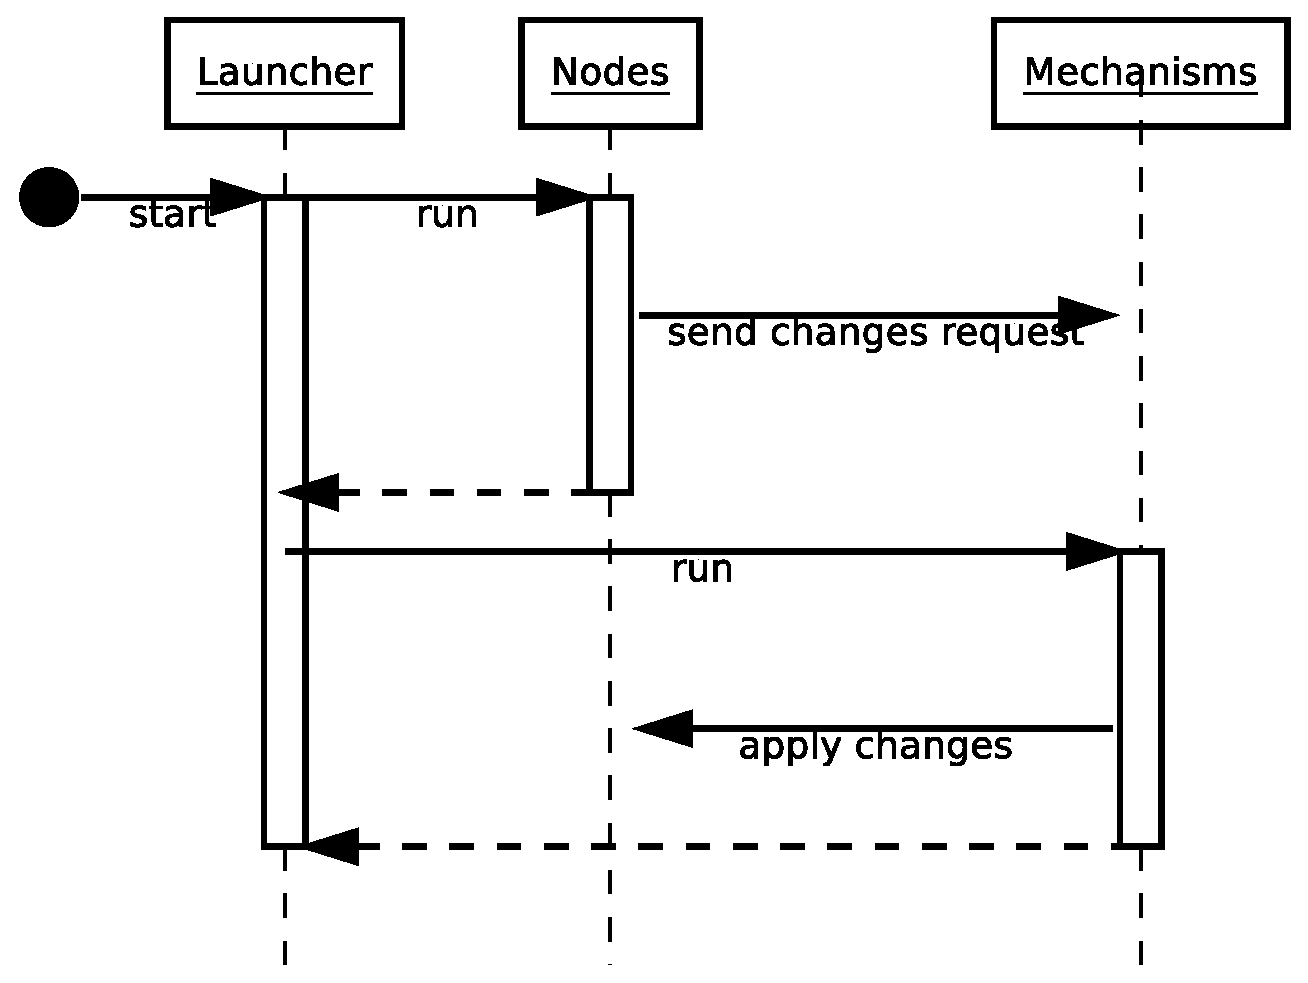
\includegraphics[width=0.7\linewidth]{2_2_2_sequence_diag}}
    \caption{Принцип работы класса \textit{abstract\_launcher}}
    \label{im:2_2_2_sequence_diag}
\end{figure}

Реализация механизмов синхронизации является ключевым звеном в разработке архитектуры данного фреймворка. Предполагается, что система работает в рамках одного адресного пространства и отдельные компоненты могут исполняться в отдельных потоках. Поскольку механизмы являются средством взаимодействия между модулями так же предполагается, что количество обращений к данным классам достаточно высоко и поэтому блокирующий вызов может существенно понизить отклик всей системы.

\begin{figure}[h]
    \centering{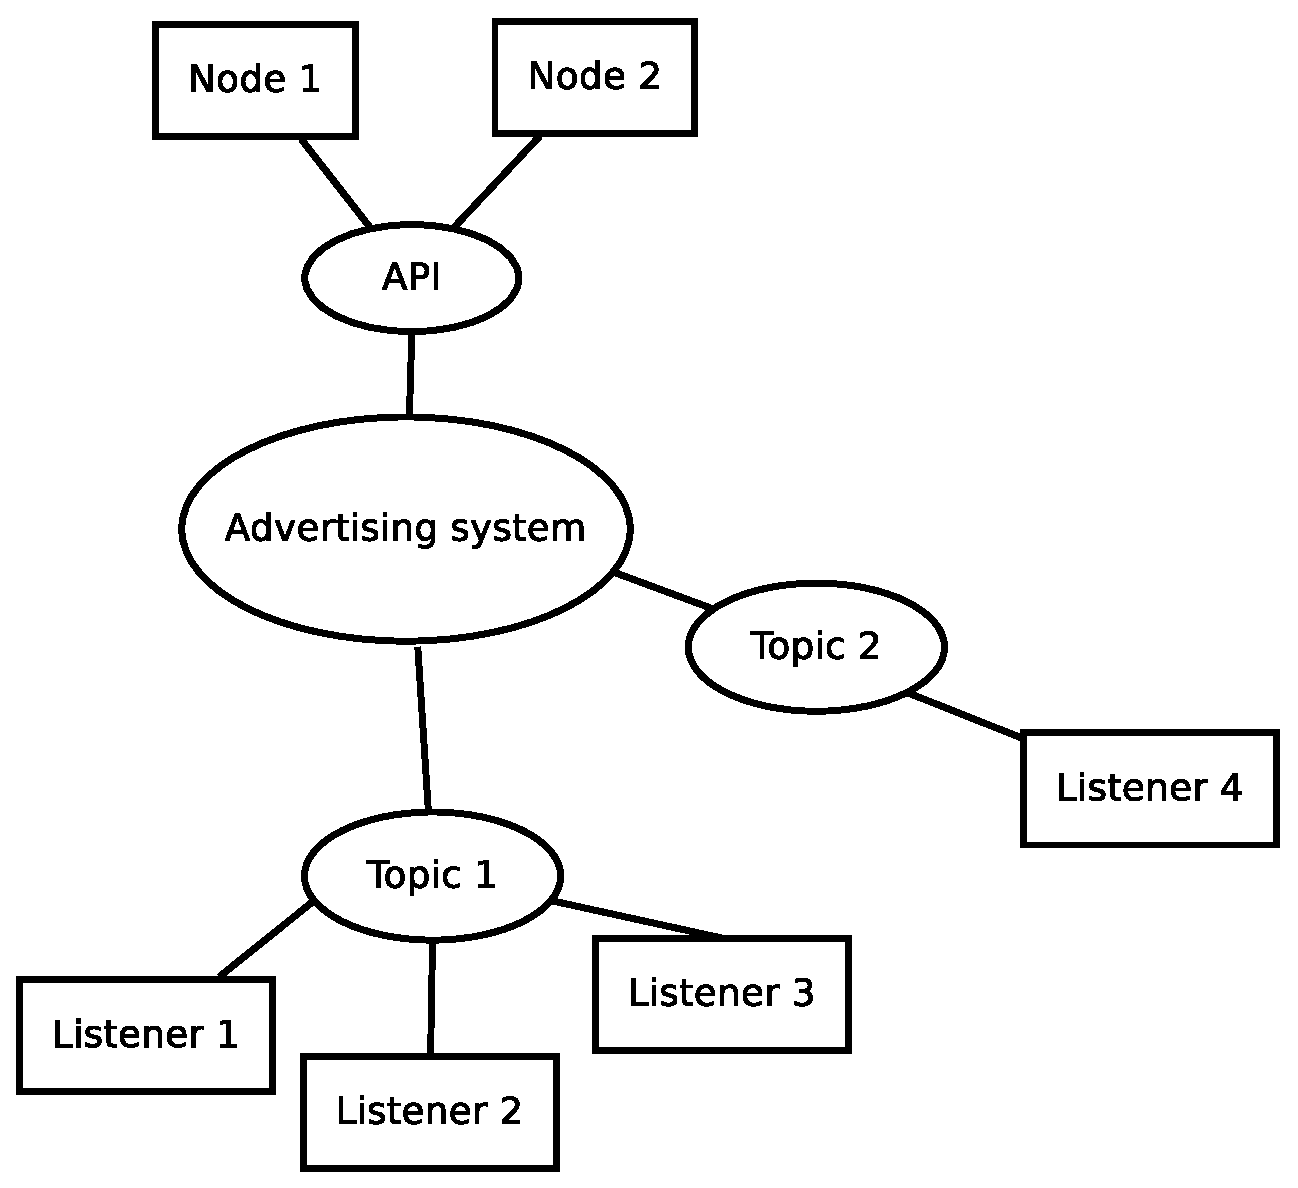
\includegraphics[width=0.7\linewidth]{2_2_3_topic}}
    \caption{Система рассылки сообщений}
    \label{im:2_2_3_topic}
\end{figure}

На рис. \ref{im:2_2_3_topic} схемматически изображен граф системы рассылки сообщений с двумя модулями, двумя топиками и четырьмя слушателями. На данном графике <<механизм>> выступает в роли API доступа к системе рассылки. Ребра графа показывают наличие возможности прямого вызова между компонентами системы круглые вершины обозначают компонент ядра системы, а прямоугольные - компоненты, реализованные пользователем.

Интерфейс системы рассылки сообщений включает в себя четыре функции: отправить сообщение в топик, получить список топиков, добавить слушателя сообщений в топик и удалить слушателя из топика. Топик может существовать только если у него есть хотя бы один подписчик - это требуется для освобождения памяти при удалении подписчиков.

Далее будут расмотренны различные варианты взаимодействия модулей с механизмом синхронизации на примере данной структуры в ситуации, когда модули обрабатываются параллельно.





\section{Проектирование асинхронного фреймворка}

При проектировании асинхронной модели фреймворка была существенно изменена архитектура синхронного ядра. Так же при проектировании были учтены выявленные архитектурные ошибки в синхронных версиях. Данная реализация системы подразумевает использование высокоскоростных алгоритмов десериализации. При тестировании данной системы исползовалась библиотека Google Flat Buffers, но данная реализация позволяет применять любой алгоритм сериализации/десериализации с использованием бинарного буфера памяти.

Отличие асинхронной версии от синхронной в первую очередь заключается в том, что система сама уведомляет о всех изменениях: модули регистрируют функции обратного вызова для получения требуемой информации о состоянии системы при ее изменениях.

\begin{figure}[h]
    \centering{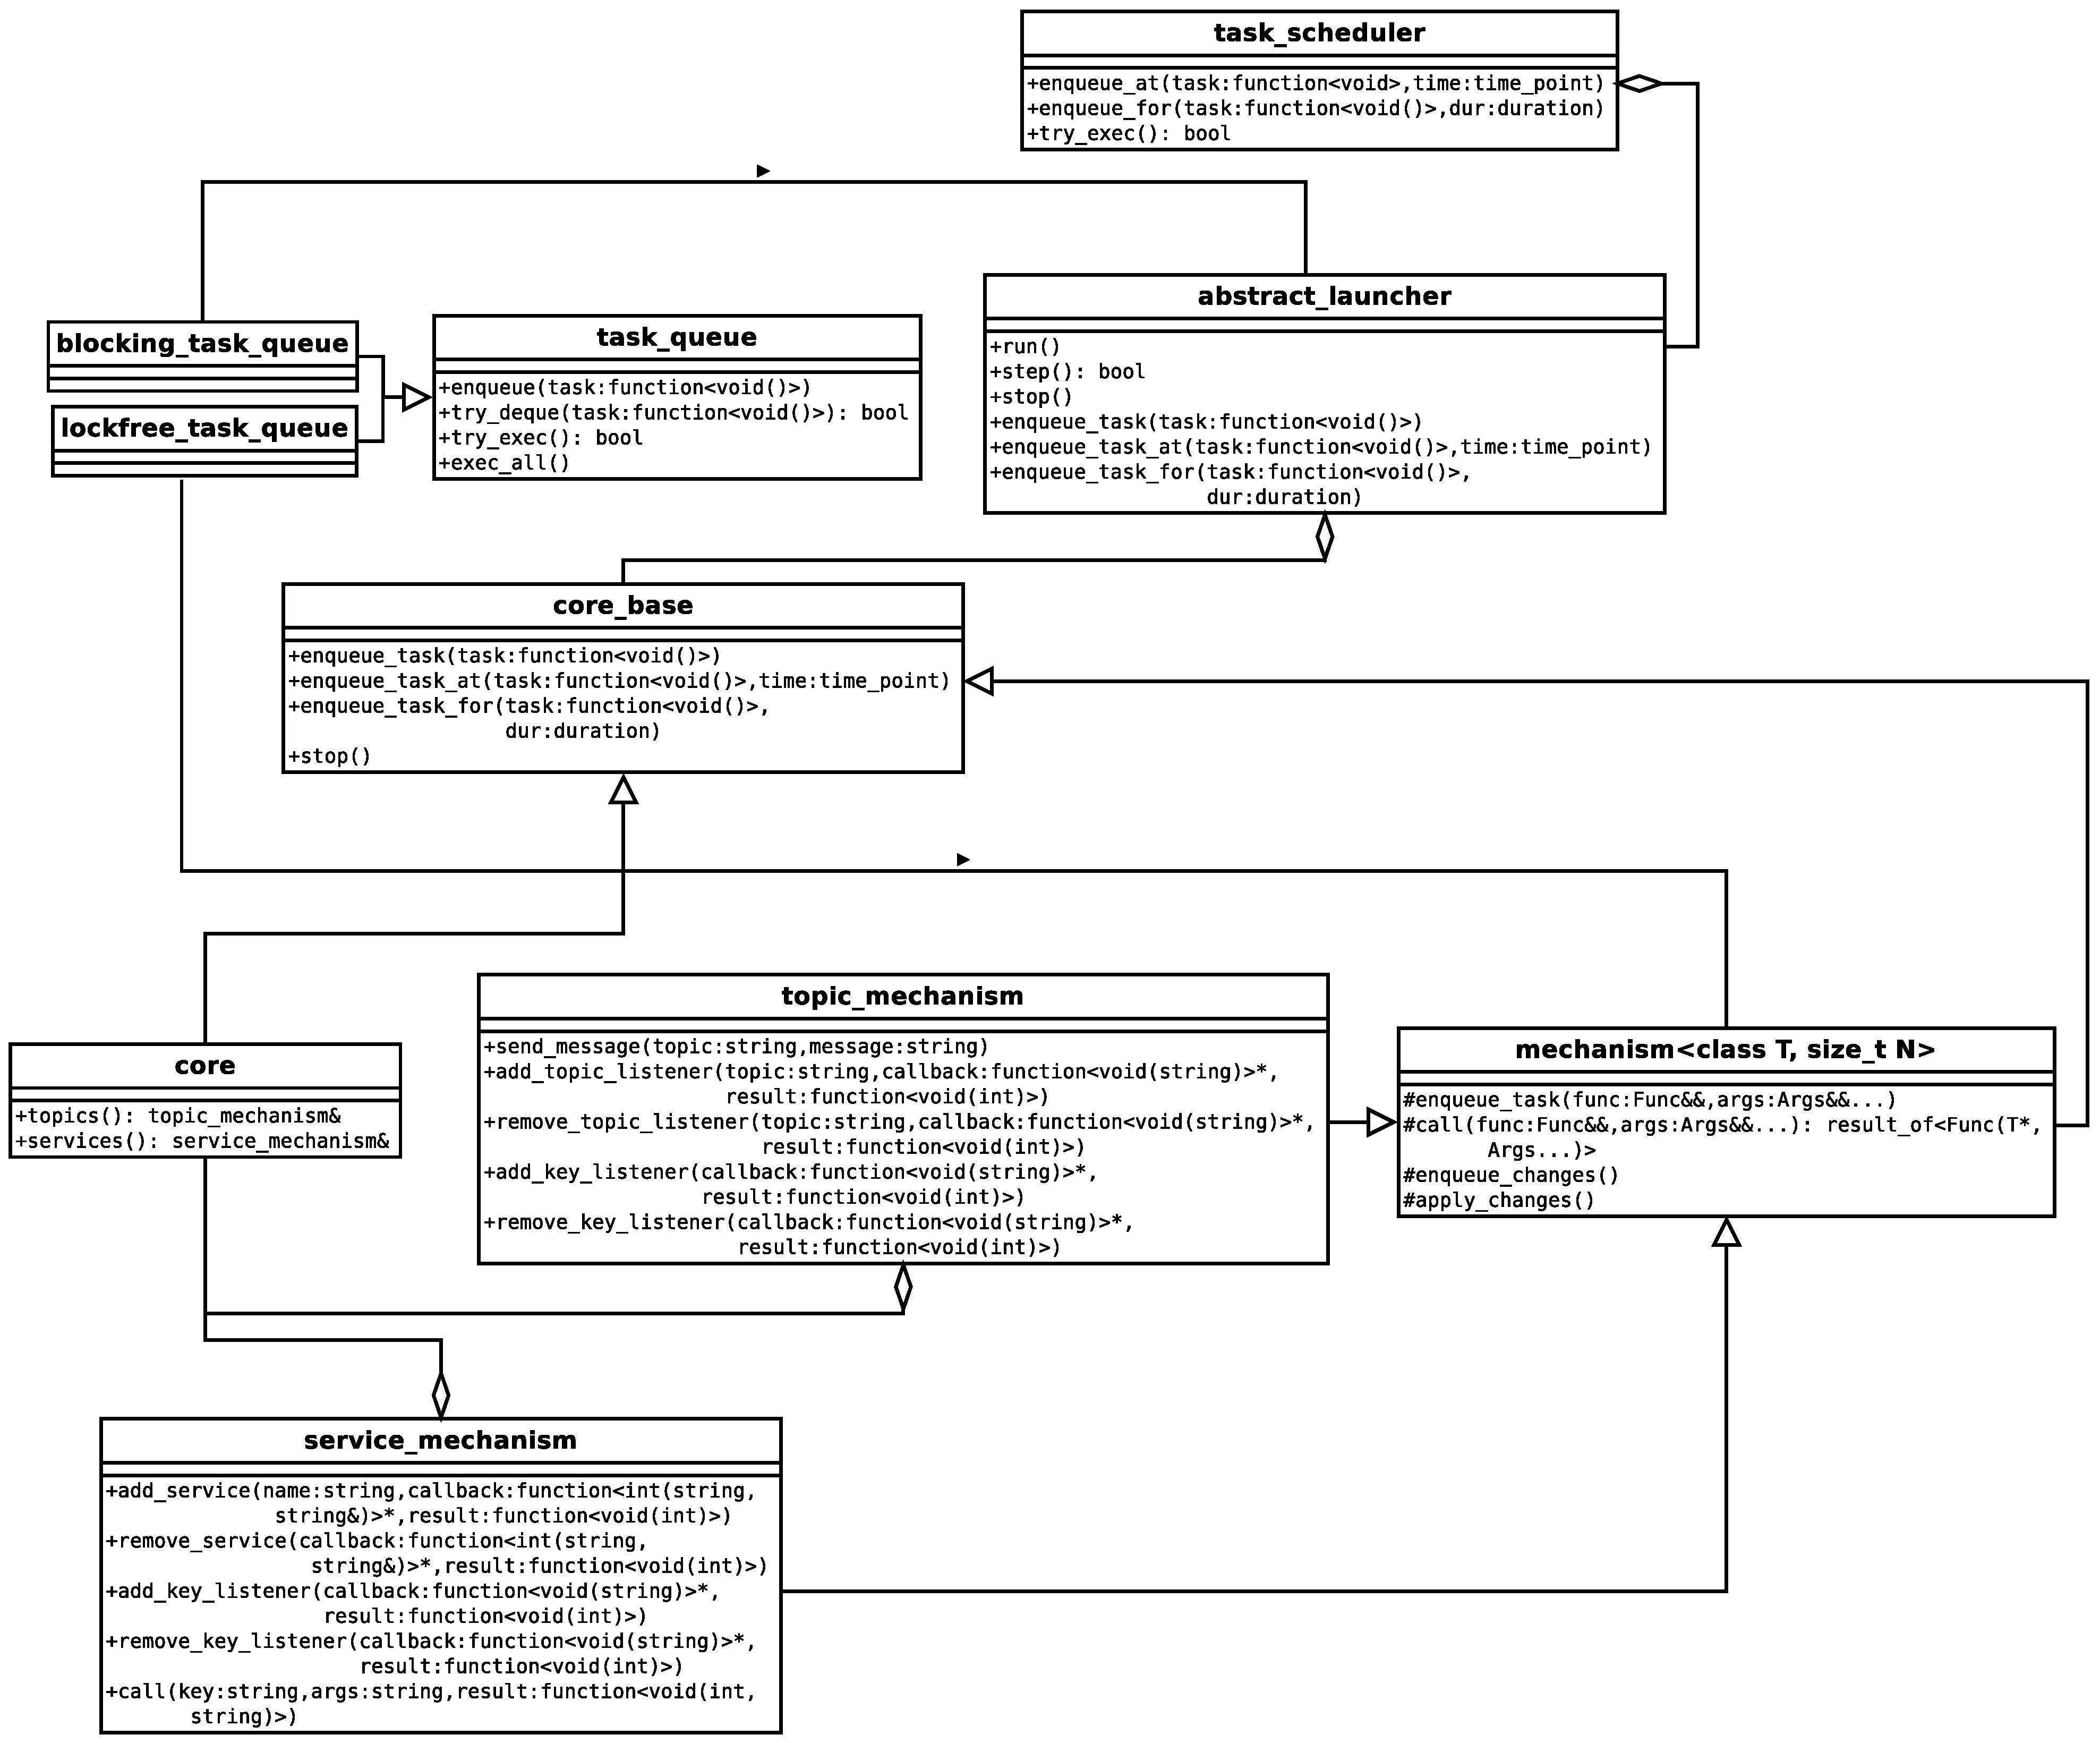
\includegraphics[width=1\linewidth]{2_3_1_async}}
    \caption{Диаграмма классов асинхронной версии фреймворка}
    \label{im:2_3_1_async}
\end{figure}

\textit{abstract\_launcher} --- задачи данного класса схожи с аналогичным классом из синхронной версии фреймворка: класс определяет порядок и способ исполнения задач. Синхронная версия расширенна функциями планировщика для выполнения задачи в определенный момент времени или спустя заданный промежуток времени. Обращения к этому классу могут происходить напрямую из разных потоков и поэтому реализация должна учитывать данный фактор.

\textit{task\_scheduler} --- класс, который позволяет добавлять задачи на исполнение в определенный момент времени. Планировщик основан на потокобезопасной очереди с приоритетами: каждая задача хранит дополнительную информацию о моменте времени, после которого она может быть получена из очереди и исполнена.

\textit{task\_queue} --- роль интерфейса очереди задач схожа с \textit{absract\_queue\_adapter} в синхронной версии. Поскольку в системе потокобезопасные очереди используютя исключительно для хранения отложенных для исполнения задач, интерфейс был адаптирован для этих целей.

\textit{lockfree\_task\_queue} --- компонент, реализуюший интерфейс абстрактной очереди задач с использованием потокобезопасной очереди без блокировок.

\textit{blocking\_task\_queue} --- компонент, реализуюший интерфейс абстрактной очереди задач с использованием потокобезопасной очереди без блокировок.

\textit{core\_base} --- базовый класс ядра системы, который предоставляет модулям системы ограниченный набор методов класса \textit{abstract\_launcher} чтобы исключить повторный запуск системы и использует очереди без блокировок для увеличения производительности при конкурентном добавлении задач без использования планировщика.

\textit{core} --- класс, который расширяет базовый класс ядра и включает в себя набор механизмов, который будет в дальнейшем использоваться модулями. Класс позволяет добавлять и удалять механизмы в систему без существенных изменений API.

\textit{mechanism} --- интерфейс механизма, предоставляющий потокобезопасную обертку вокруг потоконебезопасного класса. Из-за большого количества нюансов при асинхронном исполнении подробное описание реализаций данного класса и его наследников предоставленно ниже.

\textit{topic\_mechanism} --- компонент, реализующий механизм коммуникации между модулями путем рассылки сообщений. Данный механизм реализован по аналогии с системой рассылки сообщений в ROS.

\textit{service\_mechanism} --- компонент, реализующий механизм коммуникации между модулями с использованием отложенного вызова метода по имени. Вызовы происходят в неблокирующем режиме, поэтому система позволяет отправить несколько запросов до получения ответа. Аргументы метода передаются в структуре сообщения.

\begin{figure}[h]
    \centering{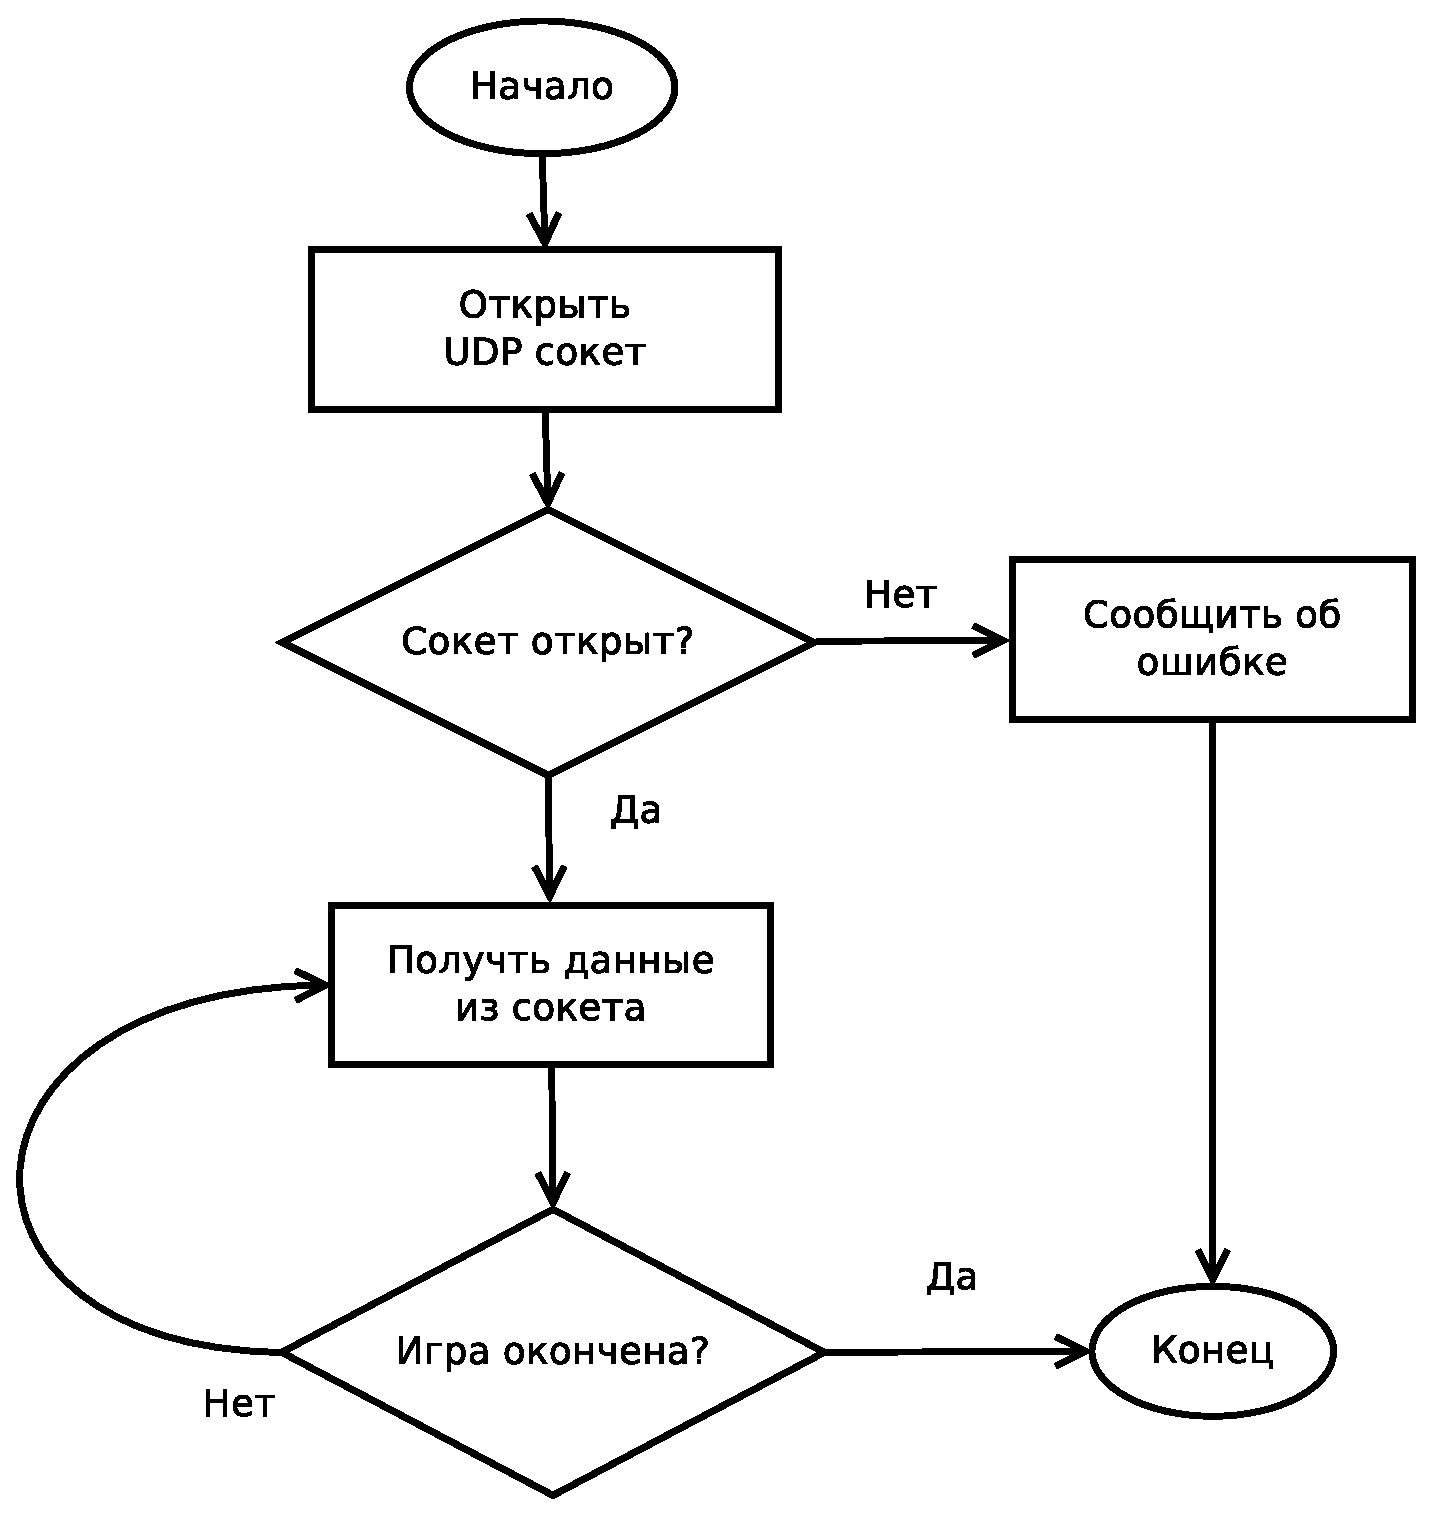
\includegraphics[width=0.5\linewidth]{2_3_2_gc}}
    \caption{Последовательность действий при взаимодействием с игровым контроллером}
    \label{im:2_3_2_gc}
\end{figure}

В данной реализации отсутствует класс нода из-за особенностей архитектуры. Каждый модуль можно описать группой методов, которые выполняются в определенном порядке и при определенных условиях. Данные методы можно обернуть в экземпляр функционального объекта и добавлять их в очередь задач при необходимости. Для примера можно взять модуль взаимодействия через сетевое соединение с игровым контроллером туртира RoboCup (рис. \ref{im:2_3_2_gc}): для взаимодействия используется UDP сокет, на который приходят данные о состоянии игры. В данном модуле можно выделить три метода, которые описывают все возможные действия: открыть UDP сокет, получить данные из сокета и сообщить об ошибке. Если сокет был успешно открыт, то в очередь задач добавляется функтор, отвечающий за получение данных из сокета, в противном случае в очередь задач добавляется функтор, отвечающий за обработку ошибки. По аналогии создаются функторы для других стадий алгоритма.

Такой подход к описанию модуля позволяет разбить его выполнение на множество небольших методов, которые зависят друг от друга, что в свою очередь уменьшает вероятность блокирование очереди задач одним модулем на длительный промежуток времени. При этом данный подход имеет два существенных недостатка: асинхронное приложение гораздо сложнее поддается отладке и требуется дополнительные расходы на аллокацию памяти под функторы и добавление в глобальную очередь задач, что может понизить производиетнльность всей системы при большом количестве задач.

В случае исполнения задач в пуле потоков отсутствует возможность обеспецить потокобезопасное исполнение модуля без блокировок и без дополнительных абстракций, которые существенно усложнили бы структуру всей системы. Из этого следует, что в данной реализации для потокобезопасного исполнения модулей без дополнительных примитивов внутри самих модулей разработчик должен гарантировать, что в очереди задач находится только одна задача одного модуля при условии, что система не будет обрабатывать функции обратного вызова при изменении состояния.

В асинхронной версии библиотеки существенно измененны механизмы синхронизации. В их основе все также лежат потокобезопасные очереди без блокировок с отложенными вызовами функций. В одном механизме может существовать несколько очередей синхронизации для упорядочивания асинхронных вызовов к механизму, например, сначала идет обработка запросов на изменение количества слушателей, после идет отправка сообщений на данные слушатели. В каждом механизме существует метод добавления в лаунчер задачи на применение изменений. Данный метод гарантирует, что задача на обновление добавлена в лаунчер только один раз, чтобы уменить потерю производительности, и все задачи будут выполнены в одном потоке.

Поскольку механизм использует функции обратного вызова существует вероятность, что эти функторы могут после выполнения добавлять в механизм новые задачи, что может привести к блокировки всей системы из-за того, что механизм будет работать бесконечно, постоянно добавляя себе новые задачи. Данная проблема решается ограничением количества вызовов за одну итерацию обработки входящих событий из очереди. Если во время исполнения был превышен лимит, то механизм повторно добавляет в очередь задачу обновления механизма.

На сегодняшний день существует асинхронная версия библиотеки для языка C++ с блокирующей синхронизацией, с помощью которой можно разработать подобную модульную систему - Boost Asio \cite{torjo2013boost}. Поскольку библиотека показывает достаточно высокие показатели производительности для асинхронной библиотеки, поддерживается большим сообществом разработчиков, то в рамках работы не планируется проектирование асинхронного фреймворка с блокирующей синхронизацией. В результатах тестирования быстродействия приведены сравнительные результаты производительности межмодульного взаимодействия и скорости исполнения очереди задач для асинхронного фреймворка с синхронизацией без блокировок и Boost Asio.







\section*{Выводы по главе 2}
\addcontentsline{toc}{section}{Выводы по главе 2}